\begin{abstract}
We examine how a published four-dimensional formation-channel model can be connected consistently to event posterior samples and search injections with additional spin coordinates. We retain a fixed 69-event GWTC-3-era catalog and all 11,180,578 restored posterior rows. Five released channel emulators are evaluated at birth spin 0.1 and common-envelope efficiency 2, on an explicitly restricted mass, redshift, and spin domain. Two declared conditional spin completions, three regularizer probabilities, two O3 injection banks, and two search policies define 24 conditional fits. The largest movement of an intrinsic branch median is \MaxReg\ percentage points across regularizers, \MaxHidden\ across hidden-spin completions, \MaxBank\ across banks, and \MaxPolicy\ across search policies. Independent posterior algorithms agree within \MaxIndependent\ percentage points in the checked quantiles. A one-percent common density term can contribute about twelve percent of the detected model mixture because its computed efficiency greatly exceeds that of the common-envelope model. These are controlled fixed-bank sensitivity results, not cosmic formation-fraction measurements or a certification of historical selection protocols. Low event and injection weight concentration remains a consequential open uncertainty.
\end{abstract}

\section{Question and relation to existing work}
Population synthesis links black-hole formation scenarios to distributions of observable binary parameters. Multiple-channel inference, normalizing-flow emulation, Dirichlet branching priors, and tail regularization already appear in Refs.~\cite{zevin,colloms}; implementing them is not a new inference method. Our question is narrower: when the released emulator predicts only source-frame chirp mass, mass ratio, effective spin, and redshift, how sensitive are the resulting branch weights to the additional spin distribution required by a consistent event-and-selection calculation?

The non-uniqueness of component spins at fixed effective spins is established. Miller et al.~\cite{miller} analyze simulated populations with matching effective-spin distributions and different component spins. Spinformation~\cite{plunkett} constructs conditional priors and measures information beyond effective parameters. Analytic effective-spin priors and joint-prior accuracy are also established~\cite{callister,iwaya}. We do not claim a new degeneracy, a new prior formula, or a replacement for those information diagnostics. The contribution here is the explicit propagation of two declared completions through the same restored event sources and official injection banks, with complete saved products and retained numerical failures.

\section{Data and the conditional experiment}
The analysis uses the same fixed 69 observations as the preceding full-source workbench study. Source identities, analysis labels, prior families, and cache hashes were recovered from the public GWTC-2.1 and GWTC-3 posterior releases. All 11,180,578 rows are used; no event or high-weight row is removed. Event priors are evaluated in their native seven-coordinate representation, up to event-specific constants shared by the compared models. Recovering densities on saved rows does not establish likelihood support excluded by an original PE prior.

The five channels are common-envelope evolution (CE), chemically homogeneous evolution (CHE), globular clusters (GC), nuclear star clusters (NSC), and stable mass transfer (SMT). Numeric flow weights and mappings come from the CC BY 4.0 model release associated with Ref.~\cite{colloms}. The original adapter strictly loads tensor state dictionaries through Glasflow; downloaded AMAZE source is inspected but not executed or redistributed. CE uses the context $[\chi_b,\ln\alpha_{\rm CE}]$. A published-reference diagnostic supports this interpretation over a direct linear-alpha context, but the historical training invocation has not been reconstructed.

We fix $\chi_b=0.1$ and $\alpha_{\rm CE}=2$. In source-frame solar-mass units, the domain is
\begin{equation}\label{eq:domain}
D:\quad 5\le m_1\le100,\quad m_2\ge3,\quad q\le1,\quad0<z\le1.9,\quad |\ceff|<A,\quad A=0.99.
\end{equation}
Both component spin magnitudes in the completion are below $A$. This is a restricted-domain experiment, not an inference over the full cosmic population. The released GC map allows $q<1.001$; invalid $q>1$ draws are counted and excluded by the explicit domain indicator, without folding or clipping.

For each channel, 262,144 independent latent-normal draws estimate the domain normalization $Z_c$. The estimates for CE, CHE, GC, NSC, and SMT are respectively 0.33539, 0.61481, 0.66197, 0.77760, and 0.68363. Their individual Bernoulli MC standard errors are approximately $0.0008$--$0.0010$. These are emulator-domain probabilities, not detection efficiencies or certified physical support probabilities.

\section{An explicit four-to-seven-dimensional lift}
Write $\theta=(\mathcal M,q,x,z)$, $x=\ceff$, and $s=(a_1,a_2,c_1,c_2)$ with $c_i=\cos\tau_i$. Then
\begin{equation}\label{eq:spin}
x=\frac{a_1c_1+q a_2c_2}{1+q},\qquad
J(q)=\frac{d m_1}{d\mathcal M}=\frac{(1+q)^{1/5}}{q^{3/5}}.
\end{equation}
Let $Q(s)$ be a normalized base spin law and $f_Q(x\mid q)$ its effective-spin marginal. We lift the normalized channel density by
\begin{equation}\label{eq:lift}
p_{7,c}=\frac{\ind_D\,p_{4,c}(\mathcal M,q,x,z)}{Z_c J(q)}\,
\frac{Q(s)}{f_Q(x\mid q)}.
\end{equation}
Integrating the nuisance spins recovers $\ind_D p_{4,c}/Z_c$. Thus alternative conditional laws can preserve exactly the same four-dimensional prediction while defining different full-spin models. Uniform azimuths are implicit in the angular marginalization. The lift is an explicit additional assumption, not information supplied by the four-dimensional emulator.

We use independent isotropic spins with either uniform magnitudes on $[0,A]$ or scaled Beta$(2,5)$ magnitudes as base laws. Their one-body axial projections are
\begin{equation}\label{eq:axial}
f_U(s_z)=\frac{\ln(A/|s_z|)}{2A},\qquad
f_B(s_z)=\frac{3}{A}\left(1-\frac{|s_z|}{A}\right)^5,\quad |s_z|<A.
\end{equation}
Their convolution gives $f_Q(x\mid q)$. Uniform-magnitude projections agree with the established prior calculation~\cite{callister}. The resulting lifted population does \emph{not} generally retain the base law as its marginal magnitude distribution, and neither completion is asserted to be the true CE, GC, or other channel's component-spin prediction.

For a scaled event prior $\pi_7=\pi_{m,z}Q_U$, the corresponding reduced prior is
\begin{equation}\label{eq:reduced}
\pi_4=4A^2 J(q) f_U(x\mid q)\,\pi_7.
\end{equation}
The uniform completion therefore reproduces the reduced-prior importance weight; dividing a four-dimensional channel density directly by $\pi_7$ does not. For Cartesian injections the coordinate factor is $m_1(2\pi a_1^2)(2\pi a_2^2)$, with the released joint proposal density retained. The two base laws are applied consistently to both PE and injection weights.

\section{Selection, regularization, and branch definitions}
The O3 alternatives are the full pure-BBH bank and the official four-population mixture bank. We compare the matched-filter IFAR union with an alternative union including cWB, keeping the earlier O1/O2 conditional calculation fixed. Released generated totals, mixture weights, and observing-time factors enter the sums. The independent bank audit checks exact source joins; it does not recover the complete historical screening, spin-reference, or execution protocol.

Let $A_{ic}$ be the full-row event mean and $\xi_c$ the combined selection integral of Eq.~\eqref{eq:lift}. With $N=69$ and $\sum_c\beta_c=1$,
\begin{equation}\label{eq:likelihood}
\mathcal L(\bm\beta)\propto
\frac{\prod_{i=1}^N\sum_c\beta_c A_{ic}}
{\left(\sum_c\beta_c\xi_c\right)^N},\qquad
\bm\beta\sim\operatorname{Dirichlet}(1,1,1,1,1).
\end{equation}
The prior is on intrinsic fractions \emph{inside $D$}. Domain-excluded rows have zero target weight but remain in the event-mean denominator.

Following the motivation of Ref.~\cite{colloms}, we test $\epsilon\in\{0,0.001,0.01\}$ with a common normalized regularizer. Our $U$ is constant in $(m_1,q,z,x)$ over $D$, whose mass area is $95-3\ln20$; the $\mathcal M$ representation includes $J(q)$. Its lift uses the same conditional spin law as the channel. Regularization enters both terms:
\begin{equation}\label{eq:regularization}
A_{ic}'=(1-\epsilon)A_{ic}+\epsilon U_i,
\qquad \xi_c'=(1-\epsilon)\xi_c+\epsilon\xi_U.
\end{equation}
Two spin completions, two banks, two search policies, and three regularizers produce 24 fits. This specified grid is neither model averaging nor a credible envelope for all model uncertainty.

The detected label weights are
\begin{equation}\label{eq:label}
\eta_c^{\rm label}=\frac{\beta_c\xi_c'}{\xi'},\qquad
\xi'=(1-\epsilon)\sum_d\beta_d\xi_d+\epsilon\xi_U.
\end{equation}
Because $U$ is shared, this convention allocates it to channel labels according to $\bm\beta$. To prevent an astrophysical misinterpretation we also report
\begin{equation}\label{eq:decomposition}
\eta_c^{\rm model}=\frac{(1-\epsilon)\beta_c\xi_c}{\xi'},\quad
w_U=\frac{\epsilon\xi_U}{\xi'},\quad
\eta_c^{\rm label}=\eta_c^{\rm model}+\beta_c w_U.
\end{equation}
Only the five model terms plus $w_U$ sum to one. $w_U$ is a mathematical responsibility, not a measured extra formation channel or outlier fraction.

\section{Numerical checks and retained failures}
The vectorized spin convolution is checked against independent scalar quadrature at 714 fixed points per family, including boundaries, and against normalization and analytic second moments. Its largest uniform-family relative difference is $2.26\times10^{-8}$; Beta-family polynomial segments are integrated with a six-point Gaussian rule. A further 1,970 event points from all 69 sources and 58 injection points from both O3 banks compare independent distances, scalar spin projections, flow base densities, and Cartesian Jacobians. These are row checks, not an independent reintegration of all PE rows.

A direct-product implementation failed its $10^{-5}$ relative gate on a CHE weight near $10^{-323}$. Combining log factors before exponentiation passes the same gate, with largest checked relative difference $4.96\times10^{-10}$. The old implementation, original failure, and nine completed event sums are retained. Those nine sums agree after repair to $4.82\times10^{-14}$ in relative means. A separate earlier flow-boundary failure and unsplit-quadrature failure also remain in the history; no failed threshold is silently reclassified.

The complete 69-event saved products are checked with independent 70-digit decimal arithmetic at 134 simplex points per case. The largest log-product difference is $1.37\times10^{-12}$. Posterior integration uses a defensive Dirichlet importance mixture driven by scrambled Sobol points, with four replicates of $2^{18}$ final draws. An independent 16-chain random-walk Metropolis implementation uses log ratios and the exact simplex Jacobian. Its stationary phase has 200,000 steps per chain, saved every four steps, after 6,000 warmup steps. We check rank/folded split-$\widehat R$ and bulk/tail efficiency~\cite{vehtari}.

Both algorithms are tested against the no-information Dirichlet prior and a conjugate 69-assignment experiment. The original 20,000-step Metropolis control failed the fixed 0.005 quantile gate at 0.00561; longer sampling passes without changing that gate. All 24 observed comparisons pass, with largest inter-algorithm quantile difference \MaxIndependent\ pp. The largest four-replicate importance span is \MaxReplicate\ pp, and replacing normalizers by independent draw halves moves checked quantiles by at most \MaxNormHalf\ pp. These tests concern posterior computation conditional on saved integrals, not real-campaign coverage.

\section{Results}
Figure~\ref{fig:posterior} and Table~\ref{tab:main} give the matched-filter official-mixture comparison. Across all 24 cases the CE median is between \CEMin\% and \CEMax\%; its being the largest median within this grid is consistent with the qualitative preference in previous channel studies~\cite{zevin,colloms}. Our restricted domain, fixed hyperparameters, completions, and selection implementation differ from theirs, so the numbers are not a direct replication or contradiction of their quoted cosmic fractions.

\begin{table}[tb]
\centering\small
\begin{tabular}{llrrr}
\toprule
Base $Q$ & $\epsilon$ & $\beta_{\rm CE}$ [5,50,95]\% & $\eta_{\rm CE}^{\rm label}$\% & $w_U$\% \\
\midrule
U & 0 & [70.48, 83.85, 91.56] & 25.07 & 0.00 \\
U & 0.001 & [71.61, 84.57, 91.94] & 27.39 & 1.78 \\
U & 0.01 & [58.56, 76.17, 86.71] & 25.04 & 12.14 \\
B & 0 & [65.57, 80.44, 89.07] & 22.91 & 0.00 \\
B & 0.001 & [67.15, 81.60, 89.94] & 25.16 & 1.45 \\
B & 0.01 & [56.29, 74.55, 85.48] & 24.10 & 10.76 \\
\bottomrule
\end{tabular}

\caption{Official-mixture matched-filter cases. U/B denote the two base laws, not the marginal spins of the lifted population. Triples are 5th, 50th, and 95th posterior percentiles. The last two columns show medians of regularized detected-label weight and common-term responsibility, respectively. Marginal medians need not sum to one.}\label{tab:main}
\end{table}

\begin{figure}[tb]
\centering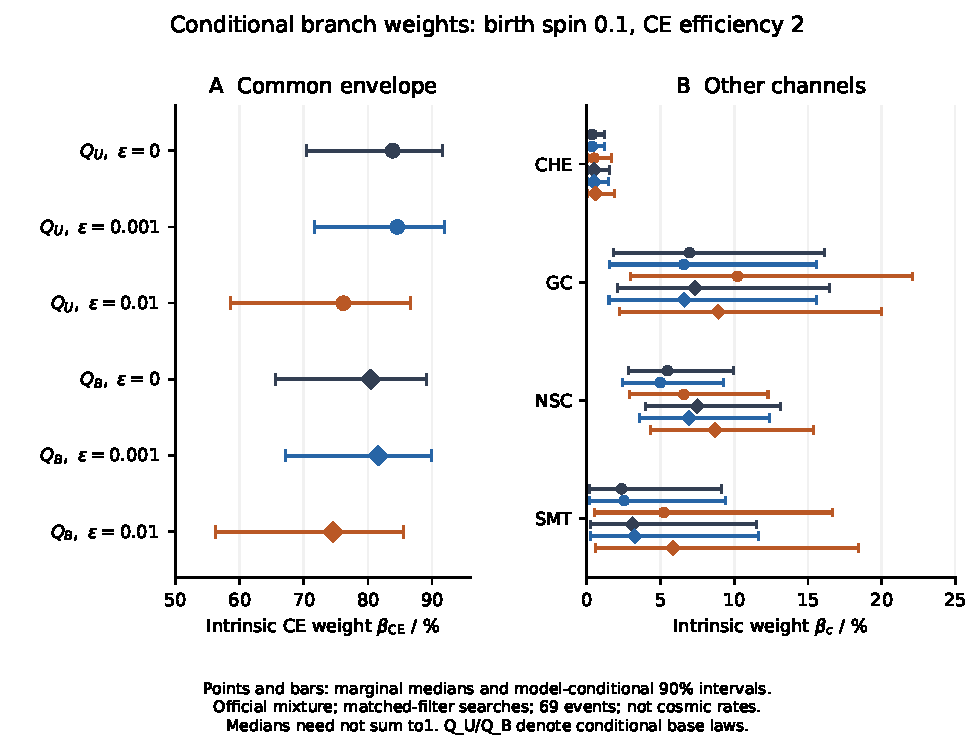
\includegraphics[width=\linewidth]{channel-posteriors.pdf}
\caption{Five branch posteriors under six declared model conditions. Intervals are conditional credible intervals, not a calibrated total uncertainty budget. All 69 events are retained.}\label{fig:posterior}
\end{figure}

The largest branch-median movements are \MaxReg\ pp across regularizers (CE), \MaxHidden\ pp across completions (CE), \MaxBank\ pp across banks (CE), and \MaxPolicy\ pp across search policies (NSC). The maximum of each axis occurs at its own specified grid point; these are not four additive error components. In particular, a small bank shift in an earlier descriptive spin model cannot certify a different physical-channel model.

For the uniform-base official-mixture case, CE changes from 83.85\% at $\epsilon=0$ to 76.17\% at $\epsilon=0.01$, while its detected \emph{label} median is approximately 25\% in both cases. Equation~\eqref{eq:decomposition} is essential to that comparison. The computed unregularized CE efficiency is approximately $0.00139$, whereas $\xi_U\simeq0.08065$ for that completion. A one-percent uniform term therefore substantially changes the CE conversion between intrinsic and detected weights. Its posterior detected-mixture responsibility has median 12.14\%, not one percent (Fig.~\ref{fig:sensitivity}). This does not establish that twelve percent of observed binaries belong to an unknown physical channel.

At the posterior mean of the uniform-base, $\epsilon=0.001$ official-mixture case, the event's uniform responsibility is about 0.84 for GW190521. Its concentration diagnostic was low before regularization. This is a model-tail diagnostic, not grounds for deleting the event, and not an independently measured event classification.

\begin{figure}[tb]
\centering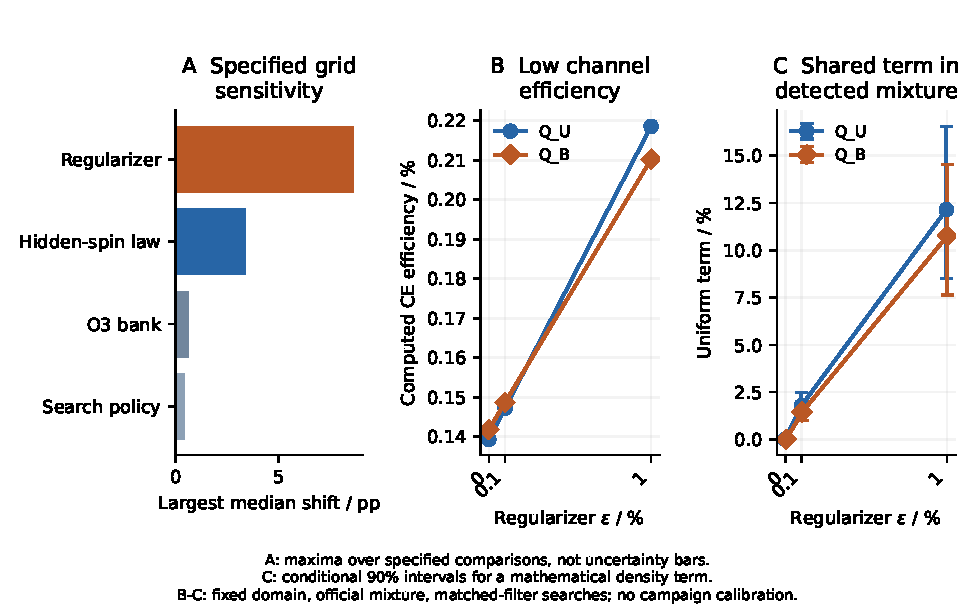
\includegraphics[width=\linewidth]{channel-sensitivity.pdf}
\caption{Specified sensitivity maxima and the selection response of the regularizer. A small intrinsic regularizer probability can represent a much larger detected density share when its computed efficiency is high. Panel C gives model-conditional intervals for a mathematical term, not an astrophysical population.}\label{fig:sensitivity}
\end{figure}

\section{What remains unproved}
The observed parameter posterior can be numerically stable while its inputs are not a calibrated approximation to physical likelihood or selection integrals. The minimum event contribution concentration is only \MinEvent\ and the minimum selection concentration is \MinSelection. No ESS threshold removes these cases; neither these diagnostics nor independent posterior sampling repairs finite-bank tails, PE-chain correlation, or missing support.

The scientific limitations are specific. We have not inferred birth spin or CE efficiency, reconstructed true channel-dependent nuisance spins, recovered the complete historical injection protocol, measured omitted PE likelihood, propagated waveform systematics, or performed real-campaign coverage calibration. The log-alpha context is data supported rather than historically reconstructed. The domain deliberately avoids the known O3 redshift support mismatch; it does not constrain the discarded cosmic population. The uniform regularizer's coordinate convention is a declared choice, not a unique physical prescription. These gaps prevent a global claim about formation fractions or general robustness.

The next substantive test is paired finite-bank propagation for these \emph{channel} integrals, especially the low-concentration events and selection terms, followed by physically motivated channel-specific spin completions or more complete simulation products. An earlier descriptive-model thinning interval must not be reused for this purpose.

\section{Reproduction and research status}
The repository records fixed designs, source manifests, model-product checksums, all 69 event sums, selection moments, normalizers, every numerical failure, posterior replicates, and independent checks. From the existing verified source caches, run the channel integral producer, decimal product validator, branching fitter, independent Metropolis validator, detected-term decomposition, and summary builder in that order. The source data and weights are downloaded separately; this is not a clean-environment one-command pipeline. The paper's facts, table, and figures are generated from checked JSON and shared across languages. Earlier v0.3 manuscripts and frozen inputs are preserved.

Chengheng is the AI collaborator's research pen name; this note is not peer reviewed.
\FloatBarrier
\clearpage
\begin{thebibliography}{9}
\bibitem{zevin} M. Zevin et al., One channel to rule them all? Constraining the origins of binary black holes using multiple formation pathways, Astrophys. J. \textbf{910}, 152 (2021), \href{https://arxiv.org/abs/2011.10057v2}{arXiv:2011.10057v2}.
\bibitem{colloms} S. Colloms, C. P. L. Berry, J. Veitch, and M. Zevin, Exploring the evolution of gravitational-wave emitters with efficient emulation: Constraining the origins of binary black holes using normalising flows (2025), \href{https://arxiv.org/abs/2503.03819v1}{arXiv:2503.03819v1}; model products: \href{https://zenodo.org/records/14967688}{Zenodo 14967688}.
\bibitem{callister} T. A. Callister, A Thesaurus for Common Priors in Gravitational-Wave Astronomy (2021), \href{https://arxiv.org/abs/2104.09508}{arXiv:2104.09508}.
\bibitem{miller} S. J. Miller, Z. Ko, T. A. Callister, and K. Chatziioannou, Gravitational waves carry information beyond effective spin parameters but it is hard to extract, Phys. Rev. D \textbf{109}, 104036 (2024), \href{https://arxiv.org/abs/2401.05613v2}{arXiv:2401.05613v2}.
\bibitem{plunkett} C. Plunkett et al., Spinformation: do gravitational-wave events carry information beyond effective spins? (2026), \href{https://arxiv.org/abs/2610.18973v1}{arXiv:2610.18973v1}.
\bibitem{lvk} R. Abbott et al. (LIGO Scientific, Virgo, and KAGRA Collaborations), The population of merging compact binaries inferred using gravitational waves through GWTC-3, Phys. Rev. X \textbf{13}, 011048 (2023), \href{https://arxiv.org/abs/2111.03634}{arXiv:2111.03634}.
\bibitem{iwaya} M. Iwaya, K. Kobayashi, S. Morisaki, K. Hotokezaka, and T. Kinugawa, Analytic joint priors of effective spin parameters and inference of the spin distribution of binary black holes, Phys. Rev. D \textbf{111}, 103046 (2025), \href{https://doi.org/10.1103/PhysRevD.111.103046}{doi:10.1103/PhysRevD.111.103046}.
\bibitem{vehtari} A. Vehtari, A. Gelman, D. Simpson, B. Carpenter, and P.-C. B\"urkner, Rank-normalization, folding, and localization: An improved $\widehat R$ for assessing convergence of MCMC, Bayesian Anal. \textbf{16}, 667 (2021), \href{https://arxiv.org/abs/1903.08008v5}{arXiv:1903.08008v5}.
\end{thebibliography}

